\documentclass{beamer}
\useoutertheme[height=10mm,width=14mm,hideallsubsections]{sidebar}
\usetheme{PaloAlto}
\usecolortheme{clover}
\setbeamercovered{transparent}
\setbeamertemplate{navigation symbols}{}
\setbeamertemplate{sections in toc}{[ball unnumbered]}
\usepackage{times}
\usefonttheme{structurebold}
\usepackage[english]{babel}
\usepackage{amsmath,amssymb,amsfonts}
\usepackage{graphicx,color,multimedia,verbatim}
\usepackage[utf8]{inputenc}
\usepackage{listings}
\usepackage{hyperref}
\usepackage{tikz}
\usepackage{gnuplot-lua-tikz}

\def\dealrelease{8.2.1}
\lstset{escapechar=\%}

\title[deal.II Overview]{deal.II: An Overview}
\author[Guido Kanschat]{Guido Kanschat}
\institute[IWR, Uni Heidelberg]{IWR, Universität Heidelberg\\[2mm]

\includegraphics[height=.2\textheight]{iwr}
\hfill

\includegraphics[height=.2\textheight]{dealclover}
\hfill
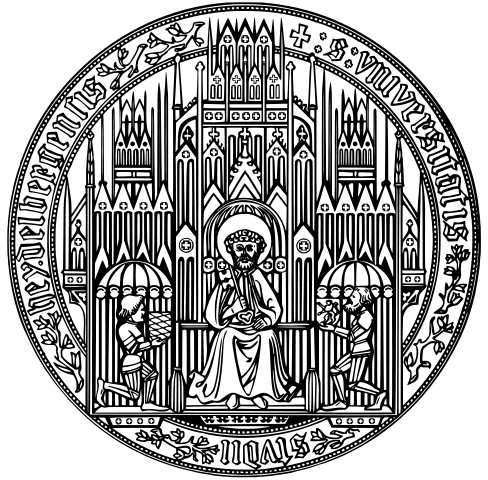
\includegraphics[height=.25\textheight]{unihd}
}
%
\pgfdeclareimage[height=10mm]{logo}{dealclover}
\logo{\pgfuseimage{logo}}
%
\def\R{\mathbb R}
\def\T{\mathbb T}                           % triangulation
\def\divh{\nabla_h\!\cdot}
\def\red{\color{red}}
\def\blue{\color{blue}}
\def\black{\color{black}}
\definecolor{green}{rgb}{0, .7, 0}
\def\green{\color{green}}
%
%\input{only}
%
\hypersetup{urlcolor=blue}
\newcommand{\myurl}[2]{\underline{\href{#1}{#2}}}
\begin{document}
\begin{frame}[plain]
  \titlepage    
\end{frame}

%%%%%%%%%%%%%%%%%%%%%%%%%%%%%%%%%%%%%%%%%%%%%%%%%%%%%%%%%%%%%%%%%%%%%%
\section{Application Examples}


\begin{frame}
  \frametitle{Euler flow downhill}
  \begin{center}
    \includegraphics[width=.31\textwidth]{pic/dealii/Gallery-Euler1}
    \includegraphics[width=.31\textwidth]{pic/dealii/Gallery-Euler2}
    \includegraphics[width=.31\textwidth]{pic/dealii/Gallery-Euler3}
  \end{center}
  
  Source: David Neckels
\end{frame}

\begin{frame}
  \frametitle{Dendrite growth}
  \begin{center}
    \includegraphics[height=.49\textwidth]{pic/dealii/Gallery-dendrite1}
    \includegraphics[height=.49\textwidth]{pic/dealii/Gallery-dendrite2}
  \end{center}

  Source: Denis Danilov
\end{frame}

\begin{frame}
  \frametitle{Advection-diffusion}
  \begin{center}
    \includegraphics[width=.49\textwidth]{pic/dealii/Advdiff}
    \includegraphics[width=.49\textwidth]{pic/dealii/Gallery-kpp}
  \end{center}
  
  Source: Orhan Mamedov, Vladimir Tomov, Abner Salgado
\end{frame}

\begin{frame}
  \frametitle{Geophysics}
  \begin{center}
    \includegraphics[width=.49\textwidth]{pic/dealii/Gallery-convection}
    \includegraphics[width=.49\textwidth]{pic/dealii/mantle-convection}
  \end{center}

  Sources: André Große-Wöhrmann, Timo Heister
\end{frame}

\begin{frame}
  \frametitle{Phase functions and immersed boundaries}
  \begin{center}
    \includegraphics[width=.49\textwidth]{pic/dealii/Immersed-bdry}
    \includegraphics[width=.49\textwidth]{pic/dealii/Gallery-Grain_growth}
  \end{center}

  Sources: Luca Heltai, Slawa
\end{frame}

\begin{frame}
  \frametitle{Plastic deformation}
  \includegraphics[width=.3\textwidth]{pic/dealii/step-18-02}
  \includegraphics[width=.3\textwidth]{pic/dealii/step-18-05}
  \includegraphics[width=.3\textwidth]{pic/dealii/step-18-07}

  \includegraphics[width=.3\textwidth]{pic/dealii/step-18-08}
  \includegraphics[width=.3\textwidth]{pic/dealii/step-18-09}
  \includegraphics[width=.3\textwidth]{pic/dealii/step-18-10}
\end{frame}

%%% Local Variables: 
%%% mode: latex
%%% TeX-master: "slides"
%%% End: 


\section{Introduction to deal.II}
\frame{\tableofcontents[currentsection,hideothersubsections]}
\subsection{History and philosophy}
%%%%%%%%%%%%%%%%%%%%%%%%%%%%%%%%%%%%%%%%%%%%%%%%%%%%%%%%%%%%%%%%%%%%%% 
\begin{frame}
  \frametitle{deal.II in a nutshell}
  \begin{center}
    
\includegraphics[height=5ex]{deallogo}
  \end{center}
  is
  \begin{itemize}
  \item a programming library in C++
  \item a toolbox for development
  \end{itemize}
  \pause
  is not
  \begin{itemize}
  \item a solver for wave/flow/radiation/electromagnetics
  \item a programming language for numerical PDE
  \end{itemize}
\end{frame}

\begin{frame}
  \frametitle{A short history of deal.II}
  \begin{description}
  \item[1990-1992] Discussion among students on simplifying the task of implementing finite element methods
  \item[1992-1997] Development of DEAL in order to support a group of PhD students in Heidelberg
  \item[1997-1998] Redesign of the whole core and publication of deal.II
  \item[1998-2012] Continuing development in a small, growing group of developers
  \item[since 2012] Transition to a community project
  \end{description}
\end{frame}

%%%%%%%%%%%%%%%%%%%%%%%%%%%%%%%%%%%%%%%%%%%%%%%%%%%%%%%%%%%%%%%%%%%%%% 
\begin{frame}
  \frametitle{deal.II developers (probably incomplete)}
  \begin{itemize}
  \item deal.II transitions from a group project to a
    community project
  \item \footnotesize Contributors: Moritz Allmaras, Michael Anderson,
    Wolfgang Bangerth, Andrea Bonito, Markus Bürg, John Burnell, Brian
    Carnes, Ivan Christov, Chih-Che Chueh, Marco Engelhard, Patrick Esser, Jörg
    Frohne, Joscha Gedicke, Thomas Geenen, Martin Genet, Christian Goll, Ralf
    Hartmann, Eric Heien, Timo Heister, Luca Heltai, Bärbel Janssen,
    Xing Jin, Oliver Kayser-Herold, Seungil Kim, Benjamin Shelton
    Kirk, Angela Klewinghaus, Katharina Kormann, Martin Kronbichler,
    Tobias Leicht, Yan Li, Vijay Mahadevan, Matthias Maier, Cataldo
    Manigrasso, Andrew McBride, Scott Miller, Helmut Müller, Stefan
    Nauber, David Neckels, M. Sebastian Pauletti, Jean-Paul Pelteret,
    Jonathan Pitt, Adam Powell IV, Florian Prill, Daniel Castanon
    Quiroz, Michael Rapson, Thomas Richter, Abner Salgado-Gonzalez,
    Anna Schneebeli, Jan Schrage, Ralf B. Schulz, Noman Shakir, Jason Sheldon,
    Michael Stadler, Martin Steigemann, Franz-Theo Suttmeier, Habib
    Talavatifard, Christophe Trophime, Yaqi Wang, Sven Wetterauer,
    Joshua White, Toby D. Young
  \end{itemize}
\end{frame}

%%%%%%%%%%%%%%%%%%%%%%%%%%%%%%%%%%%%%%%%%%%%%%%%%%%%%%%%%%%%%%%%%%%%%%
\begin{frame}
  \frametitle{Assessment of user base}
  \begin{itemize}
  \item Free downloads, free redistribution
    \begin{itemize}
    \item no reliable numbers
    \end{itemize}
  \item Discussion group
    \begin{itemize}
    \item 705 members (June 2016)
    \end{itemize}
  \item Github statistics (June 2016)
    \begin{itemize}
    \item 169 forks
    \item Release 8.4.1: 1212 downloads in three months
    \item Release 8.3.0: 6444 downloads since 8/2015
    \item Release 8.2.1: 4333 downloads since 1/2015
    \end{itemize}
  \item Citations of various papers
    % 697 + 324 + 92 + 
    \begin{itemize}
    \item approx 1200 (Google Scholar)
    \end{itemize}
  \end{itemize}
\end{frame}

%%%%%%%%%%%%%%%%%%%%%%%%%%%%%%%%%%%%%%%%%%%%%%%%%%%%%%%%%%%%%%%%%%%%%% 
\begin{frame}
  \frametitle{Goals of deal.II}
  \begin{enumerate}
    \item<+-> Research
  \begin{itemize}
  \item aid developing and testing new numerical algorithms
    \begin{itemize}
    \item Provide full control over all aspects of a program
    \item Be able to assess feasibility and efficiency
    \end{itemize}
  \item compromise between ease of use and efficiency
    \begin{itemize}
    \item Advanced/3D applications need high efficiency
    \item Support development of complex algorithms
    \item New algorithms for new hardware
    \end{itemize}
  \end{itemize}  
  \item<+-> Education
  \only<2->{\begin{itemize}
    \item teach a general purpose programming language
    \item provide intuitive tool for class and thesis projects
    \end{itemize}}
  \item<+-> Industrial Application
    \only<3->{\begin{itemize}
      \item Not a development goal in itself
      \item Several companies have inquired and use it
      \item Licensing: LGPL enables applicability
      \end{itemize}}
  \end{enumerate}
\end{frame}

%%%%%%%%%%%%%%%%%%%%%%%%%%%%%%%%%%%%%%%%%%%%%%%%%%%%%%%%%%%%%%%%%%%%%%
\begin{frame}
  \frametitle{Programming paradigm}
  \begin{block}{``Development by homotopy''}
    \begin{enumerate}
    \item Start with a simple application and test it
    \item Expand it step by step and test them
    \end{enumerate}
  \end{block}
  \pause
  Examples:
  \begin{itemize}
  \item<+-> From 2D to 3D
    \begin{itemize}
    \item change a template parameter
    \end{itemize}
  \item<+-> From regular to adaptive meshes
    \begin{itemize}
    \item 5 statements
    \end{itemize}
  \item<+-> From Gauss-Seidel to multigrid
    \begin{itemize}
    \item 30 statements
    \end{itemize}
  \item<+-> From sequential to multithreading
    \begin{itemize}
    \item configuration parameter
    \end{itemize}
  \item<+-> From sequential to message passing
    \begin{itemize}
    \item 20 statements
    \end{itemize}
  \end{itemize}
\end{frame}

%%%%%%%%%%%%%%%%%%%%%%%%%%%%%%%%%%%%%%%%%%%%%%%%%%%%%%%%%%%%%%%%%%%%%% 
\begin{frame}
  \frametitle{Online documentation}
  \begin{itemize}
  \item Reference manual
    \begin{itemize}
    \item Automatically generated with Doxygen
    \item approximately 550 classes
    \item more than 2200 files
    \item graphics and graphical hierarchies
    \item several thousand print pages
    \end{itemize}
  \item Tutorial
    \begin{itemize}
    \item 6 steps to an adaptive FEM solver
    \item 50+ more specialized example programs for diverse topics
    \end{itemize}
  \item Email discussion group
  \end{itemize}
\end{frame}

%%%%%%%%%%%%%%%%%%%%%%%%%%%%%%%%%%%%%%%%%%%%%%%%%%%%%%%%%%%%%%%%%%%%%% 
\begin{frame}
  \frametitle{The deal.II web page}
  \begin{center}
    \texttt{\Large\href{http://www.dealii.org}{www.dealii.org}}
  \end{center}
\end{frame}

%%% Local Variables: 
%%% mode: latex
%%% TeX-master: "slides"
%%% End: 

% $Id: features.tex 3667 2013-01-12 21:41:48Z kanschat $

%%%%%%%%%%%%%%%%%%%%%%%%%%%%%%%%%%%%%%%%%%%%%%%%%%%%%%%%%%%%%%%%%%%%%% 
\subsection{Mesh handling}
\begin{frame}
  \frametitle{Mesh handling}
  \begin{itemize}
  \item deal.II uses meshes with ``tensor product cells''
    \begin{itemize}
    \item quadrilaterals in 2D
    \item mapped hexahedra in 3D
    \end{itemize}
  \item Mappings of arbitrary order
  \item support for dimension independent programming
  \item local refinement with ``hanging nodes''
    \begin{center}
      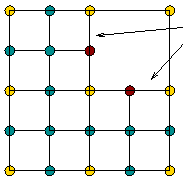
\includegraphics[height=.25\textheight]{graph/hanging}
    \end{center}
  \item storage of mesh hierarchy for multigrid
  \end{itemize}
\end{frame}

%%%%%%%%%%%%%%%%%%%%%%%%%%%%%%%%%%%%%%%%%%%%%%%%%%%%%%%%%%%%%%%%%%%%%% 
\subsection{Shape functions}
\begin{frame}
  \frametitle{Shape functions}
  \begin{itemize}
  \item $H^1$-conforming $Q_k$
  \item $H^{\text{div}}$-conforming RT$_k$, BDM$_k$
  \item $H^{\text{curl}}$-conforming Nedelec$_k$ (first family)
  \item discontinuous $Q_k$, $P_k$, vector elements
  \item support for implementation of further elements
  \end{itemize}
\end{frame}

%%%%%%%%%%%%%%%%%%%%%%%%%%%%%%%%%%%%%%%%%%%%%%%%%%%%%%%%%%%%%%%%%%%%%% 
\subsection{Degrees of freedom}
\begin{frame}
  \frametitle{Degrees of freedom}
  \begin{itemize}
  \item Element ``topology'' gets converted to ``global degrees
    of freedom''
  \item Generalized $hp$-methods
  \item Constraint operators for hanging nodes
  \item Level hierarchies of arbitrary elements
  \item Generic iterators to build matrices on cells and faces
  \end{itemize}
\end{frame}

%%%%%%%%%%%%%%%%%%%%%%%%%%%%%%%%%%%%%%%%%%%%%%%%%%%%%%%%%%%%%%%%%%%%%% 
\subsection{Systems of PDE}
\begin{frame}
  \frametitle{Systems of PDE}
  \begin{itemize}
  \item ``System elements'' simplify the implementation of systems of
    PDE
    \begin{itemize}
    \item Most data handling like for single equations
    \item Only local integrators have to change
    \end{itemize}
  \item Block vectors allow separation of equations
    \begin{itemize}
    \item Block preconditioners
    \item Projection schemes
    \end{itemize}
  \end{itemize}
\end{frame}

%%%%%%%%%%%%%%%%%%%%%%%%%%%%%%%%%%%%%%%%%%%%%%%%%%%%%%%%%%%%%%%%%%%%%% 
\subsection{Linear algebra}
\begin{frame}
  \frametitle{Linear algebra}
  \begin{itemize}
  \item Vectors and sparse matrices
  \item Elimination of hanging nodes
  \item Krylov space solvers: cg, GMRES, MinRes, Bicgstab, TFQMR
  \item Point and block relaxation
    \pause
  \item Multilevel support
  \item Block systems and Schur complements
    \pause
  \item Umfpack
  \item Interfaces to Trilinos, Lapack, Petsc, Slepc
    \pause
  \item Support for matrix free linear algebra work in progress
  \end{itemize}
\end{frame}

%%%%%%%%%%%%%%%%%%%%%%%%%%%%%%%%%%%%%%%%%%%%%%%%%%%%%%%%%%%%%%%%%%%%%% 
\subsection{Pre- and postprocessing}
\begin{frame}
  \frametitle{Pre- and postprocessing}
  \begin{itemize}
  \item<+-> Input drivers for several grid generators
    \begin{itemize}
    \item BAMG, MGF, GMSH, Salome, Cubit
    \item Graphic formats: UCD, Tecplot
    \end{itemize}
  \item<+-> Graphical output split into cell patches
    \begin{itemize}
    \item Drivers for VTK, UCD, OpenDX, gnuplot, Postscript, Tecplot, SVG
    \item Output for higher order elements
    \item New backends easily implemented
    \end{itemize}
  \end{itemize}
\end{frame}

%%%%%%%%%%%%%%%%%%%%%%%%%%%%%%%%%%%%%%%%%%%%%%%%%%%%%%%%%%%%%%%%%%%%%%
\begin{frame}
  \frametitle{The main classes}
  \centering
  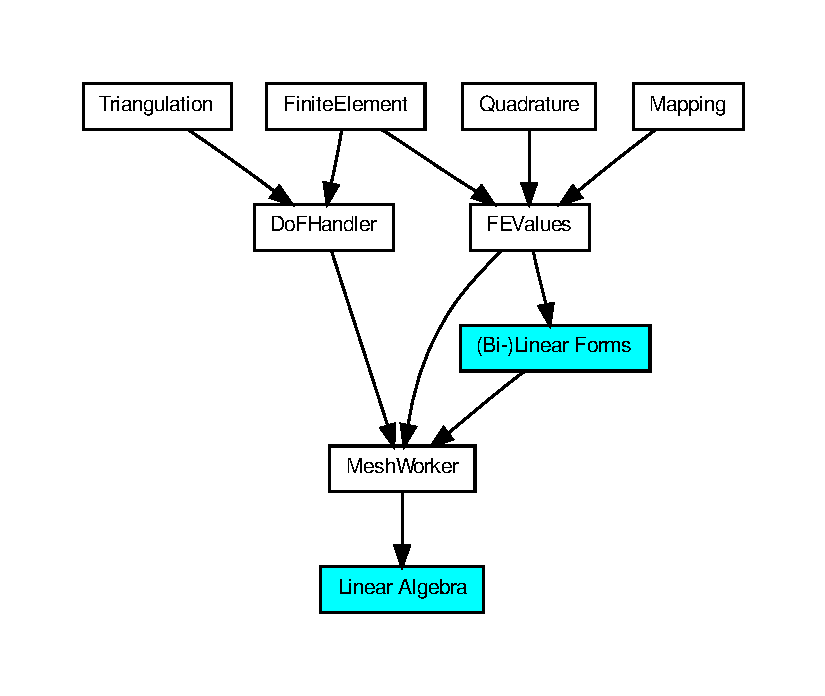
\includegraphics[height=.99\textheight]{graph/structure}
\end{frame}

%%%%%%%%%%%%%%%%%%%%%%%%%%%%%%%%%%%%%%%%%%%%%%%%%%%%%%%%%%%%%%%%%%%%%%
\begin{frame}
  \frametitle{The tutorial structure}

  \centering
  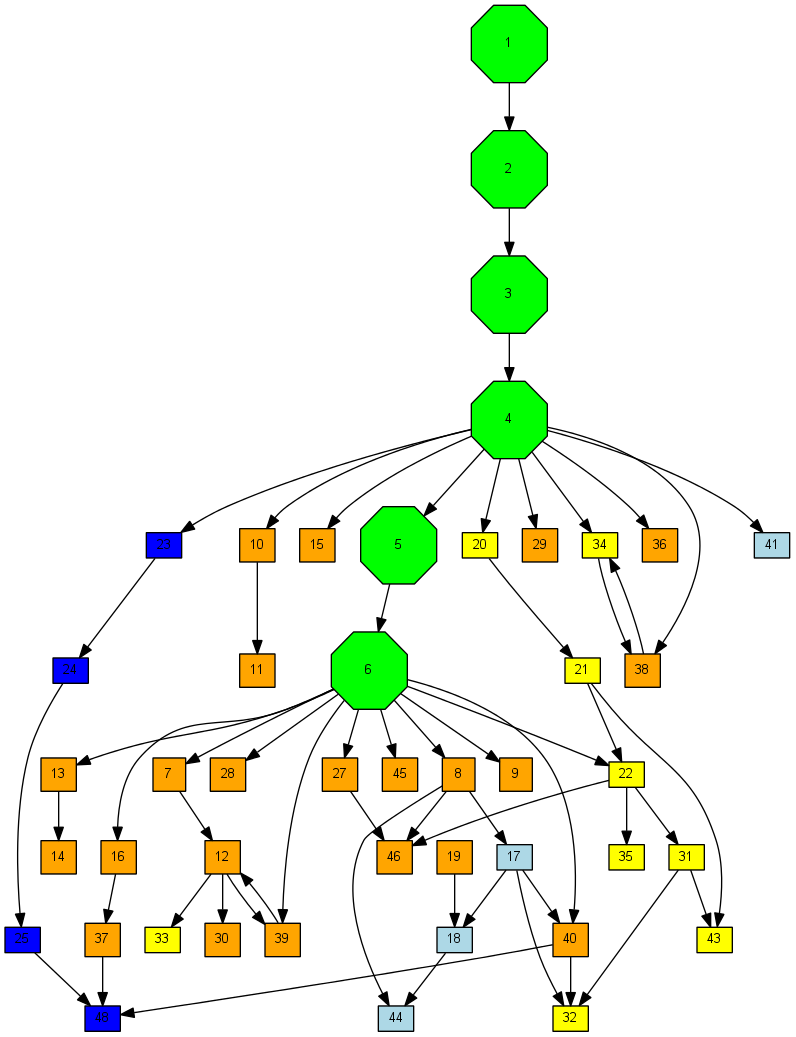
\includegraphics[height=.99\textheight]{graph/tutorial}

\end{frame}


%%% Local Variables: 
%%% mode: latex
%%% TeX-master: "slides"
%%% End: 


%%%%%%%%%%%%%%%%%%%%%%%%%%%%%%%%%%%%%%%%%%%%%%%%%%%%%%%%%%%%%%%%%%%%%%
\section[Installing]{Installing deal.II}
\frame{\tableofcontents[currentsection,hideothersubsections]}
%%%%%%%%%%%%%%%%%%%%%%%%%%%%%%%%%%%%%%%%%%%%%%%%%%%%%%%%%%%%%%%%%%%%%%
%%%%%%%%%%%%%%%%%%%%%%%%%%%%%%%%%%%%%%%%%%%%%%%%%%%%%%%%%%%%%%%%%%%%%%
\section[Virtual Box]{Setting up the virtual box}
\frame{\tableofcontents[currentsection,hideothersubsections]}

\subsection{Installing the virtual machine}
\begin{frame}
  \frametitle{Downloading the virtual machine}
  \begin{enumerate}
  \item Install the Oracle VM Virtual Box (Open Source)
    \begin{itemize}
    \item \url{www.virtualbox.org}
    \item Packaged with many Linux distributions
    \end{itemize}
  \item Download the Virtual Machine Image
    \begin{itemize}
    \item  \url{dealii.org/download.html}
    \item From USB stick provided by your instructor
    \end{itemize}
    \item Start the Virtual Box manager and import the \texttt{.ova} file
      \begin{itemize}
      \item Adjust the settings for CPUs, Memory to be less than what
        your machine has
      \item Delete the shared folder entry
      \item Check for warnings
      \end{itemize}
    \item Start the newly imported virtual image
  \end{enumerate}
\end{frame}

\subsection{Preparing dealii for our course}
\begin{frame}
  \frametitle{Preparing dealii for our course}
  \begin{enumerate}
  \item Start the terminal (second menu item in the top bar)
  \item Check for installed tutorial
    \begin{block}{}
      \lstinputlisting{code/vmsetup.sh}      
    \end{block}
  \item Edit \lstinline!setup.sh! and remove the line that contains
    \begin{block}{}
      \lstinline!git checkout v8.4.1!
    \end{block}
    \item Run \lstinline!setup.sh! 
  \item Go and have coffee, lunch, dinner, etc.
  \end{enumerate}
\end{frame}

% \subsection{Downloading and setting up amandus}
% \begin{frame}
%   \frametitle{Downloading and setting up amandus}
%   \begin{enumerate}
%   \item From your home directory, run the following:
%     \begin{block}{}
%       \lstinputlisting[basicstyle=\footnotesize]{code/vmamandus.sh}
%     \end{block}
%   \end{enumerate}
% \end{frame}

%%%%%%%%%%%%%%%%%%%%%%%%%%%%%%%%%%%%%%%%%%%%%%%%%%%%%%%%%%%%%%%%%%%%%%
%%%%%%%%%%%%%%%%%%%%%%%%%%%%%%%%%%%%%%%%%%%%%%%%%%%%%%%%%%%%%%%%%%%%%%
\section[Installing]{Installing deal.II without virtual box}
\frame{\tableofcontents[currentsection,hideothersubsections]}
\subsection{Requirements}

%%%%%%%%%%%%%%%%%%%%%%%%%%%%%%%%%%%%%%%%%%%%%%%%%%%%%%%%%%%%%%%%%%%%%%
\begin{frame}
  \frametitle{Operating system}
  \begin{itemize}
  \item Linux (e.g. Ubuntu 14.04 or higher)
    \begin{itemize}
    \item g++, 
    \end{itemize}
  \item Mac OS X
    \begin{itemize}
    \item Install current XCode or MAC Ports
    \end{itemize}
  \item Windows with Virtual Box
  \end{itemize}
  These will 
\end{frame}

%%%%%%%%%%%%%%%%%%%%%%%%%%%%%%%%%%%%%%%%%%%%%%%%%%%%%%%%%%%%%%%%%%%%%%
\begin{frame}
  \frametitle{Additional software}
  \begin{itemize}
  \item CMake (3.0 or higher)
  \item perl (5.x or higher)
  \item make or ninja as required by CMake
  \item Some visualization software
    \item Optional: 
    \begin{itemize}
    \item LAPACK, Arpack
    \item doxygen and graphviz (for documentation only)
    \item MPI, p4est (for distributed computing)
    \item Trilinos, Petsc, Slepc (parallel linear algebra)
    \end{itemize}
  \end{itemize}
\end{frame}

%%%%%%%%%%%%%%%%%%%%%%%%%%%%%%%%%%%%%%%%%%%%%%%%%%%%%%%%%%%%%%%%%%%%%%
%%%%%%%%%%%%%%%%%%%%%%%%%%%%%%%%%%%%%%%%%%%%%%%%%%%%%%%%%%%%%%%%%%%%%%
\subsection{Downloading}

%%%%%%%%%%%%%%%%%%%%%%%%%%%%%%%%%%%%%%%%%%%%%%%%%%%%%%%%%%%%%%%%%%%%%%
\begin{frame}
  \frametitle{Downloading deal.II releases}
  \begin{itemize}
  \item Go to \texttt{\myurl{http://www.dealii.org}{www.dealii.org}}
  \item In the navigation menu to the left, follow
    \myurl{http://www.dealii.org/download/index.html}{Download}
  \item Choose the release number (usually the latest)
  \item Choose the package
    \begin{itemize}
    \item Full library
    \item Premade documentation
    \end{itemize}
  \item Download the file (in \texttt{.tar.gz} format)
  \item In an appropriate place, unpack and untar the file, which will
    create a subdirectory \texttt{deal.II}.
  \end{itemize}
\end{frame}

%%%%%%%%%%%%%%%%%%%%%%%%%%%%%%%%%%%%%%%%%%%%%%%%%%%%%%%%%%%%%%%%%%%%%%
\begin{frame}
  \frametitle{Access the developing archive}
  \begin{itemize}
  \item The current state of deal.II is on github at\\
    \texttt{https://github.com/dealii/dealii.git}
  \item First time call\\
    \texttt{\footnotesize git clone https://github.com/dealii/dealii.git}
  \item make sure you regularly call\\
    \texttt{git pull}
  \item Release or subversion archive?
    \begin{itemize}
    \item Releases are tested!
    \item Archive has the most current features
    \end{itemize}
    \pause
    \item Contributing to deal.II
      \begin{itemize}
      \item Create an account and a fork on github
      \item Familiarize yourself with the git workflow
      \end{itemize}
  \end{itemize}
\end{frame}

%%%%%%%%%%%%%%%%%%%%%%%%%%%%%%%%%%%%%%%%%%%%%%%%%%%%%%%%%%%%%%%%%%%%%%
%%%%%%%%%%%%%%%%%%%%%%%%%%%%%%%%%%%%%%%%%%%%%%%%%%%%%%%%%%%%%%%%%%%%%%
\subsection{Configuring}

%%%%%%%%%%%%%%%%%%%%%%%%%%%%%%%%%%%%%%%%%%%%%%%%%%%%%%%%%%%%%%%%%%%%%%
\begin{frame}[fragile]
  \frametitle{Configuring and installing}
  \begin{itemize}
  \item Unpack library into directory of your choice
  \item Typically:
\begin{lstlisting}[language=bash,basicstyle=\ttfamily,keywordstyle=\ttfamily]
mkdir dealii
cd dealii
tar xzf /download/path/deal.II-%\dealrelease%.tar.gz
mkdir build
cd build
cmake -DCMAKE_INSTALL_PREFIX=../installed \
    ../deal.II
make install -j 4
\end{lstlisting}
\item Additional configuration options
    \begin{itemize}
    \item Disable/enable features
    \item Add interfaces to external libraries
    \item Menu with \texttt{ccmake .}
    \end{itemize}
  \end{itemize}
\end{frame}

%%%%%%%%%%%%%%%%%%%%%%%%%%%%%%%%%%%%%%%%%%%%%%%%%%%%%%%%%%%%%%%%%%%%%%
%%%%%%%%%%%%%%%%%%%%%%%%%%%%%%%%%%%%%%%%%%%%%%%%%%%%%%%%%%%%%%%%%%%%%%
\subsection{Running your first program}

%%%%%%%%%%%%%%%%%%%%%%%%%%%%%%%%%%%%%%%%%%%%%%%%%%%%%%%%%%%%%%%%%%%%%%
\begin{frame}[fragile]
  \frametitle{Running the examples}
\begin{lstlisting}[language=bash,basicstyle=\ttfamily,keywordstyle=\ttfamily]
cd dealii/installed/examples/step-1
cmake .
make run
evince grid-2.eps
\end{lstlisting}
\end{frame}


%%% Local Variables: 
%%% mode: latex
%%% TeX-master: "slides"
%%% End: 


%%%%%%%%%%%%%%%%%%%%%%%%%%%%%%%%%%%%%%%%%%%%%%%%%%%%%%%%%%%%%%%%%%%%%%
\section[Installing]{Generic loop programming}
\frame{\tableofcontents[currentsection,hideothersubsections]}
%%%%%%%%%%%%%%%%%%%%%%%%%%%%%%%%%%%%%%%%%%%%%%%%%%%%%%%%%%%%%%%%%%%%%%
%%%%%%%%%%%%%%%%%%%%%%%%%%%%%%%%%%%%%%%%%%%%%%%%%%%%%%%%%%%%%%%%%%%%%%
\subsection{Loop structures and data requirements}

%%%%%%%%%%%%%%%%%%%%%%%%%%%%%%%%%%%%%%%%%%%%%%%%%%%%%%%%%%%%%%%%%%%%%%
\begin{frame}[fragile]
  \frametitle{The assembly loop}
  \begin{gather*}
    a_{ij} = \sum_{Z\in \mathbb T_h} a(\phi_j, \phi_i)
  \end{gather*}
  \begin{block}{}
    \small
    \lstinputlisting{assembly.pseudocode}
  \end{block}  
\end{frame}

%%%%%%%%%%%%%%%%%%%%%%%%%%%%%%%%%%%%%%%%%%%%%%%%%%%%%%%%%%%%%%%%%%%%%%
\begin{frame}[fragile]
  \begin{block}{The abstract assembly loop}
    \lstinputlisting{assembly2.pseudocode}
  \end{block}
\end{frame}

%%%%%%%%%%%%%%%%%%%%%%%%%%%%%%%%%%%%%%%%%%%%%%%%%%%%%%%%%%%%%%%%%%%%%%
\begin{frame}[fragile]
  \begin{block}{The dg assembly loop}
    \lstinputlisting{assembly3.pseudocode}
  \end{block}  
\end{frame}

%%%%%%%%%%%%%%%%%%%%%%%%%%%%%%%%%%%%%%%%%%%%%%%%%%%%%%%%%%%%%%%%%%%%%%
\begin{frame}[fragile]
  \begin{block}{The vectorized dg assembly loop}
    \lstinputlisting{assembly3a.pseudocode}
  \end{block}  
\end{frame}

%%%%%%%%%%%%%%%%%%%%%%%%%%%%%%%%%%%%%%%%%%%%%%%%%%%%%%%%%%%%%%%%%%%%%%
\begin{frame}
  \frametitle{Task based parallelism by abstract loops}
  \begin{itemize}
  \item Users only provide local operators, only read local data
  \item Abstract loops enable reimplementation in the library
    \begin{itemize}
    \item Workstream with ``reliable'' accumulation, but sequential bottleneck
    \item Graph coloring and all parallel accumulation
    \item Off-loading to GPU or Xeon Phi
      \begin{itemize}
      \item Needs small code!
      \end{itemize}
    \end{itemize}
  \end{itemize}
\end{frame}


%%%%%%%%%%%%%%%%%%%%%%%%%%%%%%%%%%%%%%%%%%%%%%%%%%%%%%%%%%%%%%%%%%%%%%
\begin{frame}[fragile]
  \frametitle{FEM for linear problems}
  \begin{block}{Generic linear, stationary program}
    \lstinputlisting{linear.pseudocode}
  \end{block}
\end{frame}

%%%%%%%%%%%%%%%%%%%%%%%%%%%%%%%%%%%%%%%%%%%%%%%%%%%%%%%%%%%%%%%%%%%%%%
\begin{frame}[fragile]
  \frametitle{FEM for nonlinear problems}
  \begin{block}{Generic nonlinear, stationary program}
    \lstinputlisting{nonlinear.pseudocode}
  \end{block}
\end{frame}

%%%%%%%%%%%%%%%%%%%%%%%%%%%%%%%%%%%%%%%%%%%%%%%%%%%%%%%%%%%%%%%%%%%%%%
\begin{frame}[fragile]
  \frametitle{FEM for instationary nonlinear problems}
  \begin{block}{Generic nonlinear, instationary program}
    \lstinputlisting{timestepping.pseudocode}
  \end{block}
\end{frame}

\begin{frame}
  \frametitle{Generic loop interface in deal.II}
  \lstinline!MeshWorker! class uses three objects
  \begin{enumerate}
  \item Local operator
    \begin{itemize}
    \item  provided by user
    \end{itemize}
  \item Output object
      \begin{itemize}
      \item Matrix data
      \item Vector data
      \item Functionals and estimators
      \end{itemize}
  \item Data object
      \begin{itemize}
      \item Receives any number and any kind of (named) data
      \item Automatically evaluates finite element functions on each cell
      \end{itemize}
  \end{enumerate}
\end{frame}

\subsection{Local operators}

%%%%%%%%%%%%%%%%%%%%%%%%%%%%%%%%%%%%%%%%%%%%%%%%%%%%%%%%%%%%%%%%%%%%%%
\begin{frame}
  \frametitle{Local operators (class style)}
  \begin{block}{}
    \lstinputlisting[basicstyle=\footnotesize]{code/local_integrator.h}
  \end{block}
\end{frame}

%%%%%%%%%%%%%%%%%%%%%%%%%%%%%%%%%%%%%%%%%%%%%%%%%%%%%%%%%%%%%%%%%%%%%%
\begin{frame}
  \frametitle{Examples for local operators}
  \begin{block}{Laplace matrix}
    \lstinputlisting[basicstyle=\footnotesize]{code/laplace_matrix.h}
  \end{block}
\end{frame}

%%%%%%%%%%%%%%%%%%%%%%%%%%%%%%%%%%%%%%%%%%%%%%%%%%%%%%%%%%%%%%%%%%%%%%
\begin{frame}
  \frametitle{Examples for local operators}
  \begin{block}{The lambda version}
    \lstinputlisting[basicstyle=\footnotesize]{code/laplace_lambda.h}
  \end{block}
\end{frame}

%%%%%%%%%%%%%%%%%%%%%%%%%%%%%%%%%%%%%%%%%%%%%%%%%%%%%%%%%%%%%%%%%%%%%%
\begin{frame}
  \frametitle{Examples for local operators}
  \begin{block}{Allen-Cahn Jacobian}
    \lstinputlisting[basicstyle=\footnotesize]{code/allencahn_matrix.h}
  \end{block}
\end{frame}

%%%%%%%%%%%%%%%%%%%%%%%%%%%%%%%%%%%%%%%%%%%%%%%%%%%%%%%%%%%%%%%%%%%%%%
\begin{frame}
  \frametitle{Examples for local operators}
  \begin{block}{Allen-Cahn residual}
    \lstinputlisting[basicstyle=\footnotesize]{code/allencahn_residual.h}    
  \end{block}
\end{frame}

%%%%%%%%%%%%%%%%%%%%%%%%%%%%%%%%%%%%%%%%%%%%%%%%%%%%%%%%%%%%%%%%%%%%%%
\begin{frame}[t]
  \frametitle{Assembling the matrix}
  \lstinputlisting[basicstyle=\footnotesize]{code/matrix.cc}
\end{frame}

%%%%%%%%%%%%%%%%%%%%%%%%%%%%%%%%%%%%%%%%%%%%%%%%%%%%%%%%%%%%%%%%%%%%%%
\begin{frame}[t]
  \frametitle{Assembling the multilevel matrices}
  \lstinputlisting[basicstyle=\footnotesize]{code/mgmatrix.cc}
\end{frame}

%%%%%%%%%%%%%%%%%%%%%%%%%%%%%%%%%%%%%%%%%%%%%%%%%%%%%%%%%%%%%%%%%%%%%%
\begin{frame}[t]
  \frametitle{Assembling the right hand side}
  \lstinputlisting[basicstyle=\footnotesize]{code/rhs.cc}
\end{frame}



\section{Example}
% $Id: example.tex 2782 2011-07-25 16:39:35Z kanschat $

\lstset{language=C++,
  basicstyle=\scriptsize,%\ttfamily,
  keywordstyle=\bfseries,
  showtabs=false,
  showspaces=false,
  tabsize=2}

\subsection{Tutorial Step 16}
\begin{frame}
  \frametitle{Example: tutorial step 16}
  \begin{itemize}
  \item Solve a Poisson problem
  \item Error estimation and local refinement
  \item Continuous elements with hanging nodes
  \item Multigrid solver
  \end{itemize}
\end{frame}

%%%%%%%%%%%%%%%%%%%%%%%%%%%%%%%%%%%%%%%%%%%%%%%%%%%%%%%%%%%%%%%%%%%%%%
\begin{frame}
  \frametitle{The main class (functions)}
  \lstinputlisting{code/class1.cc}
\end{frame}

%%%%%%%%%%%%%%%%%%%%%%%%%%%%%%%%%%%%%%%%%%%%%%%%%%%%%%%%%%%%%%%%%%%%%%
\begin{frame}
  \frametitle{The main class (data)}
  \lstinputlisting{code/class2.cc}
\end{frame}

%%%%%%%%%%%%%%%%%%%%%%%%%%%%%%%%%%%%%%%%%%%%%%%%%%%%%%%%%%%%%%%%%%%%%%
\begin{frame}
  \frametitle{The main class (multigrid)}
  \lstinputlisting{code/class3.cc}
\end{frame}

%%%%%%%%%%%%%%%%%%%%%%%%%%%%%%%%%%%%%%%%%%%%%%%%%%%%%%%%%%%%%%%%%%%%%%
\begin{frame}
  \frametitle{The main class (declaration)}
  \lstinputlisting[basicstyle=\tiny,numberstyle=\tiny,numbers=left,numbersep=0pt,stepnumber=1]{code/class.cc}
\end{frame}

%%%%%%%%%%%%%%%%%%%%%%%%%%%%%%%%%%%%%%%%%%%%%%%%%%%%%%%%%%%%%%%%%%%%%%
\begin{frame}
  \frametitle{The constructor}
  \lstinputlisting{code/constructor.cc}
\end{frame}

%%%%%%%%%%%%%%%%%%%%%%%%%%%%%%%%%%%%%%%%%%%%%%%%%%%%%%%%%%%%%%%%%%%%%%
\begin{frame}
  \frametitle{Setting up the system}
  \lstinputlisting{code/setup.cc}
\end{frame}

%%%%%%%%%%%%%%%%%%%%%%%%%%%%%%%%%%%%%%%%%%%%%%%%%%%%%%%%%%%%%%%%%%%%%%
\begin{frame}
  \frametitle{Boundary and hanging node constraints}
  \lstinputlisting{code/constraints.cc}
\end{frame}

%%%%%%%%%%%%%%%%%%%%%%%%%%%%%%%%%%%%%%%%%%%%%%%%%%%%%%%%%%%%%%%%%%%%%%
\begin{frame}[t]
  \frametitle{Assembling the matrix}
  \lstinputlisting{code/matrix.cc}
\end{frame}

%%%%%%%%%%%%%%%%%%%%%%%%%%%%%%%%%%%%%%%%%%%%%%%%%%%%%%%%%%%%%%%%%%%%%%
\begin{frame}[t]
  \frametitle{Assembling the multilevel matrices}
  \lstinputlisting{code/mgmatrix.cc}
\end{frame}

%%%%%%%%%%%%%%%%%%%%%%%%%%%%%%%%%%%%%%%%%%%%%%%%%%%%%%%%%%%%%%%%%%%%%%
\begin{frame}[t]
  \frametitle{Assembling the right hand side}
  \lstinputlisting{code/rhs.cc}
\end{frame}

%%%%%%%%%%%%%%%%%%%%%%%%%%%%%%%%%%%%%%%%%%%%%%%%%%%%%%%%%%%%%%%%%%%%%%
\begin{frame}[t]
  \frametitle{Solving the linear system}
  \lstinputlisting{code/solve2.cc}
\end{frame}

%%%%%%%%%%%%%%%%%%%%%%%%%%%%%%%%%%%%%%%%%%%%%%%%%%%%%%%%%%%%%%%%%%%%%%
\begin{frame}[t]
  \frametitle{Setting up the preconditioner}
  \lstinputlisting[basicstyle=\tiny]{code/solve1.cc}
\end{frame}

%%%%%%%%%%%%%%%%%%%%%%%%%%%%%%%%%%%%%%%%%%%%%%%%%%%%%%%%%%%%%%%%%%%%%%
\begin{frame}[t]
  \frametitle{Output}
  \lstinputlisting{code/output.cc}
\end{frame}

%%%%%%%%%%%%%%%%%%%%%%%%%%%%%%%%%%%%%%%%%%%%%%%%%%%%%%%%%%%%%%%%%%%%%%
\begin{frame}[t]
  \frametitle{The outer loop}
  \lstinputlisting{code/run.cc}
\end{frame}

%%%%%%%%%%%%%%%%%%%%%%%%%%%%%%%%%%%%%%%%%%%%%%%%%%%%%%%%%%%%%%%%%%%%%%
\begin{frame}[t]
  \frametitle{The function ``main''}
  \lstinputlisting{code/main.cc}
\end{frame}

%%%%%%%%%%%%%%%%%%%%%%%%%%%%%%%%%%%%%%%%%%%%%%%%%%%%%%%%%%%%%%%%%%%%%%
\begin{frame}[t]
  \frametitle{The cell matrix}
  \lstinputlisting{code/cell_matrix.cc}
\end{frame}

%%%%%%%%%%%%%%%%%%%%%%%%%%%%%%%%%%%%%%%%%%%%%%%%%%%%%%%%%%%%%%%%%%%%%%
\begin{frame}[t]
  \frametitle{The cell matrix}
  \lstinputlisting{code/cell_matrix2.cc}
\end{frame}

%%% Local Variables: 
%%% mode: latex
%%% TeX-master: "slides"
%%% End: 


\end{document}

%%% Local Variables: 
%%% mode: latex
%%% TeX-master: t
%%% End: 
